% 	Name		:: 	sthlm Beamer Theme  HEAVILY based on the hsrmbeamer theme (Benjamin Weiss)
%	Author		:: 	Mark Hendry Olson (mark@hendryolson.com)
%	Created		::	2013-07-31
%	Updated		::	June 18, 2015 at 08:45
%	Version		:: 	1.0.2
%	Email		:: 	hendryolson@gmail.com
%	Website		:: 	http://v42.com
%
% 	License		:: 	This file may be distributed and/or modified under the
%                  	GNU Public License.
%
%	Description	::	This presentation is a demonstration of the sthlm beamer
%					theme, which is HEAVILY based on the HSRM beamer theme created by Benjamin Weiss
%					(benjamin.weiss@student.hs-rm.de), which can be found on GitHub
%					<https://github.com/hsrmbeamertheme/hsrmbeamertheme>.


%-=-=-=-=-=-=-=-=-=-=-=-=-=-=-=-=-=-=-=-=-=-=-=-=
%
%        LOADING DOCUMENT
%
%-=-=-=-=-=-=-=-=-=-=-=-=-=-=-=-=-=-=-=-=-=-=-=-=

\documentclass[newPxFont]{beamer}
\usetheme{sthlm}
%\usecolortheme{sthlmv42}

%-=-=-=-=-=-=-=-=-=-=-=-=-=-=-=-=-=-=-=-=-=-=-=-=
%        LOADING PACKAGES
%-=-=-=-=-=-=-=-=-=-=-=-=-=-=-=-=-=-=-=-=-=-=-=-=

% подключаем кириллицу 
\usepackage[T2A]{fontenc}
\usepackage[utf8]{inputenc}
\usepackage{listings}
\usepackage{graphicx}
\usepackage{hyperref}

\usepackage{chronology}

\renewcommand{\event}[3][e]{%
  \pgfmathsetlength\xstop{(#2-\theyearstart)*\unit}%
  \ifx #1e%
    \draw[fill=black,draw=none,opacity=0.5]%
      (\xstop, 0) circle (.2\unit)%
      node[opacity=1,rotate=45,right=.2\unit] {#3};%
  \else%
    \pgfmathsetlength\xstart{(#1-\theyearstart)*\unit}%
    \draw[fill=black,draw=none,opacity=0.5,rounded corners=.1\unit]%
      (\xstart,-.1\unit) rectangle%
      node[opacity=1,rotate=45,right=.2\unit] {#3} (\xstop,.1\unit);%
  \fi}%

%-=-=-=-=-=-=-=-=-=-=-=-=-=-=-=-=-=-=-=-=-=-=-=-=
%        BEAMER OPTIONS
%-=-=-=-=-=-=-=-=-=-=-=-=-=-=-=-=-=-=-=-=-=-=-=-=

%\setbeameroption{show notes}

%-=-=-=-=-=-=-=-=-=-=-=-=-=-=-=-=-=-=-=-=-=-=-=-=
%
%	PRESENTATION INFORMATION
%
%-=-=-=-=-=-=-=-=-=-=-=-=-=-=-=-=-=-=-=-=-=-=-=-=

\title{Семинар 2}
\subtitle{Введение в алгоритмы. Теория графов.}
%\date{\small{\jobname}}
%\date{\today}
\author{\texttt{Бирюков Владимир}}
\institute{МФТИ}

\hypersetup{
pdfauthor = {Бирюков Владимир},
pdfsubject = {},
pdfkeywords = {},
pdfmoddate= {D:\pdfdate},
pdfcreator = {}
}

\begin{document}

%-=-=-=-=-=-=-=-=-=-=-=-=-=-=-=-=-=-=-=-=-=-=-=-=
%
%	TITLE PAGE
%
%-=-=-=-=-=-=-=-=-=-=-=-=-=-=-=-=-=-=-=-=-=-=-=-=

\maketitle

%\begin{frame}[plain]
%	\titlepage
%\end{frame}

%-=-=-=-=-=-=-=-=-=-=-=-=-=-=-=-=-=-=-=-=-=-=-=-=
%
%	TABLE OF CONTENTS: OVERVIEW
%
%-=-=-=-=-=-=-=-=-=-=-=-=-=-=-=-=-=-=-=-=-=-=-=-=

\section{Введение в теорию графов}

%-=-=-=-=-=-=-=-=-=-=-=-=-=-=-=-=-=-=-=-=-=-=-=-=
%	TM: AT and definition
%-=-=-=-=-=-=-=-=-=-=-=-=-=-=-=-=-=-=-=-=-=-=-=-=


\begin{frame}{Граф}
\begin{columns}
\begin{column}{.48\linewidth}
Граф -- это математический объект, совокупность:
\begin{itemize}
\item $V$ = вершины
\item $E$ = ребра
\end{itemize}
Обозначается как $G = (V, E)$ \\
$n = |V|$ -- число вершин
$m = |E|$ -- число рёбер
\end{column}
\begin{column}{.48\linewidth}
		\begin{figure}
		\centerline{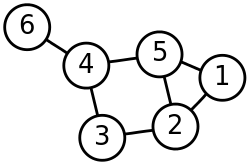
\includegraphics[width=1.0\linewidth]{images/graph1.png}}
		\end{figure}
	\end{column}
\end{columns}
\end{frame}

\begin{frame}{Граф}
\begin{columns}
	\begin{column}{.3\linewidth}
		Ориентированный
		\begin{figure}
		\centerline{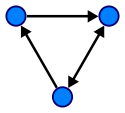
\includegraphics[width=1.0\linewidth]{images/und_graph.png}}
		\end{figure}
	\end{column}
	\begin{column}{.3\linewidth}
		Неориентированный
		\begin{figure}
		\centerline{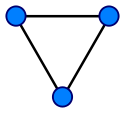
\includegraphics[width=1.0\linewidth]{images/d_graph.png}}
		\end{figure}
	\end{column}
\end{columns}
\end{frame}


\begin{frame}{Граф}
\begin{enumerate}
\item связный граф -- если для любых вершин u,v есть путь из u в v.
\item взвешенный граф -- если каждому ребру графа поставлено в соответствие некоторое число, называемое весом ребра.
\item простой граф -- если он не имеет петель и кратных рёбер.
\item ациклический граф -- если он не имеет циклов.
\item дерево -- если он связный и ациклический.
\end{enumerate}
\end{frame}

\begin{frame}{Граф. Представления. Список смежных вершин. Матрица смежности.}
\begin{figure}
\centerline{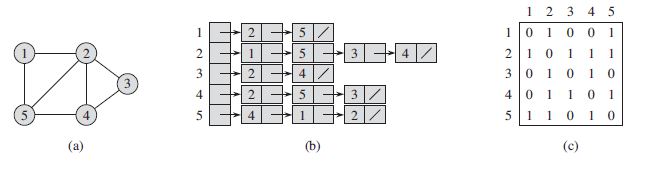
\includegraphics[width=1.1\linewidth]{images/graphrep1.png}}
\end{figure}
\end{frame}

\begin{frame}{Граф. Представления. Список смежных вершин. Матрица смежности.}
\begin{figure}
\centerline{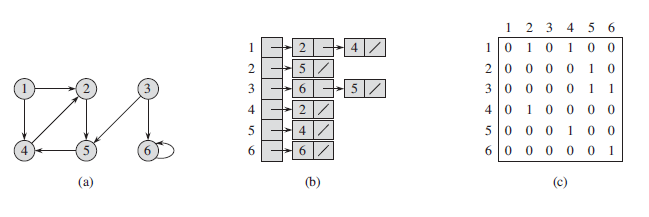
\includegraphics[width=1.1\linewidth]{images/graph_rep2.png}}
\end{figure}
\end{frame}



\begin{frame}{Граф}
\begin{columns}
	\begin{column}{.4\linewidth}
		Поиск в ширину
		\begin{figure}
		\centerline{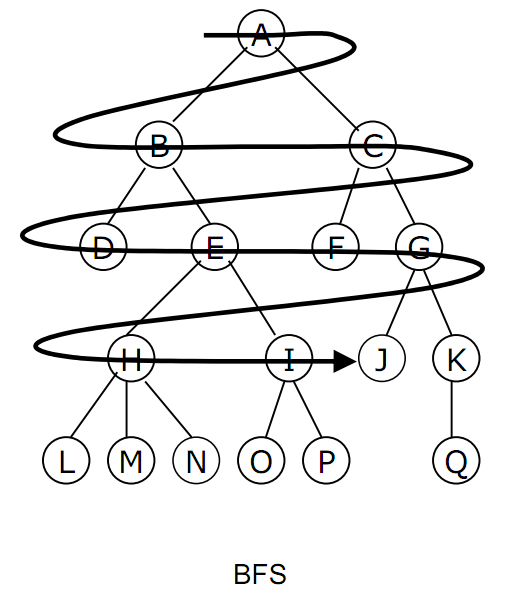
\includegraphics[width=1.0\linewidth]{images/bfs.png}}
		\end{figure}
	\end{column}
	\begin{column}{.4\linewidth}
		Поиск в глубину
		\begin{figure}
		\centerline{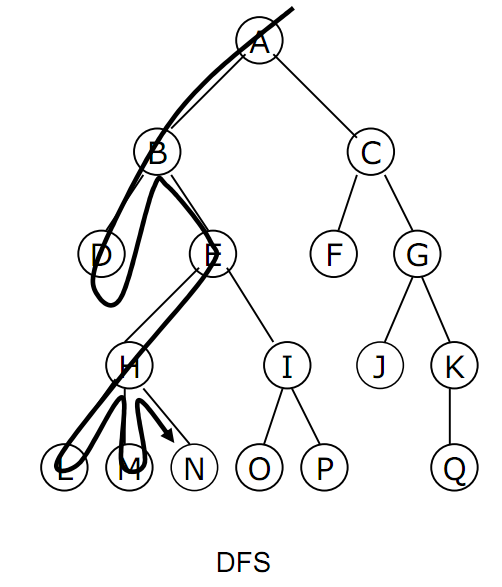
\includegraphics[width=1.0\linewidth]{images/dfs.png}}
		\end{figure}
	\end{column}
\end{columns}
\end{frame}


\begin{frame}{Граф. Псевдокод алгортма для BFS.}
\begin{figure}
\centerline{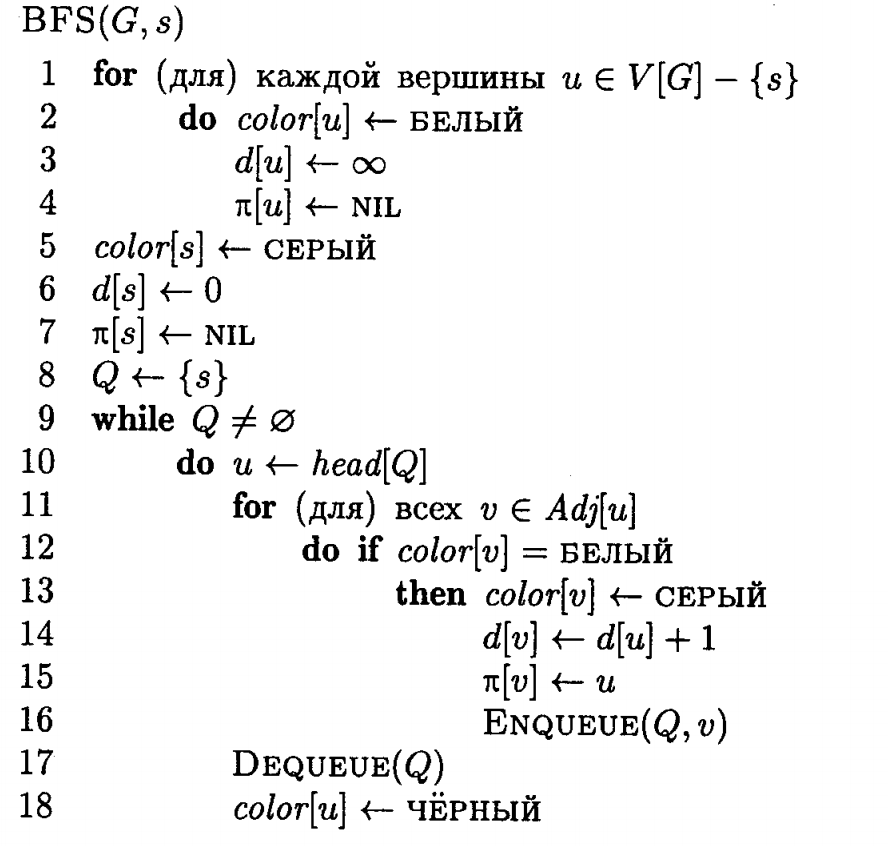
\includegraphics[width=0.7\linewidth]{images/bfs_algo.png}}
\end{figure}
\end{frame}

\begin{frame}{Граф. Алгортм BFS.}
\begin{figure}
\centerline{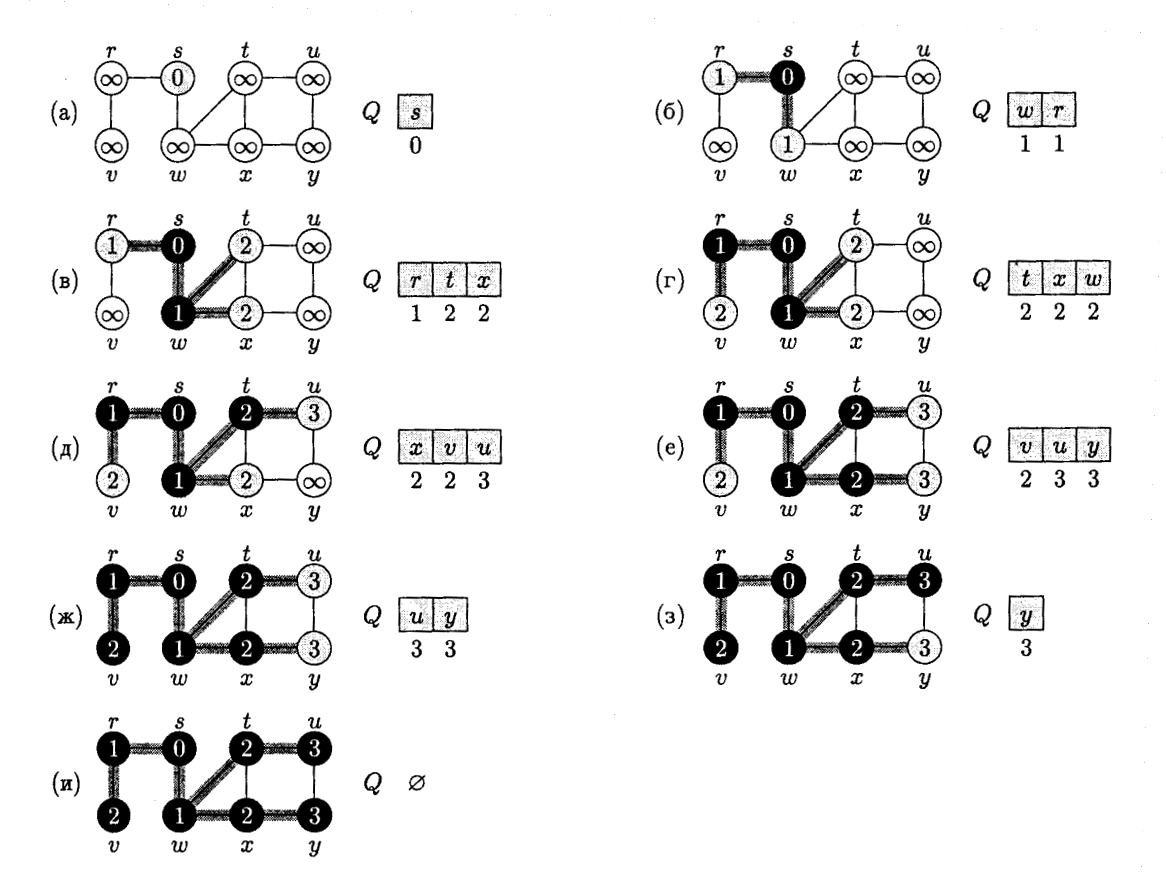
\includegraphics[width=1.0\linewidth]{images/bfs_graph.png}}
\end{figure}
\end{frame}




\begin{frame}{Граф. Кратчайшие пути из одной вершины.}
\begin{figure}
\centerline{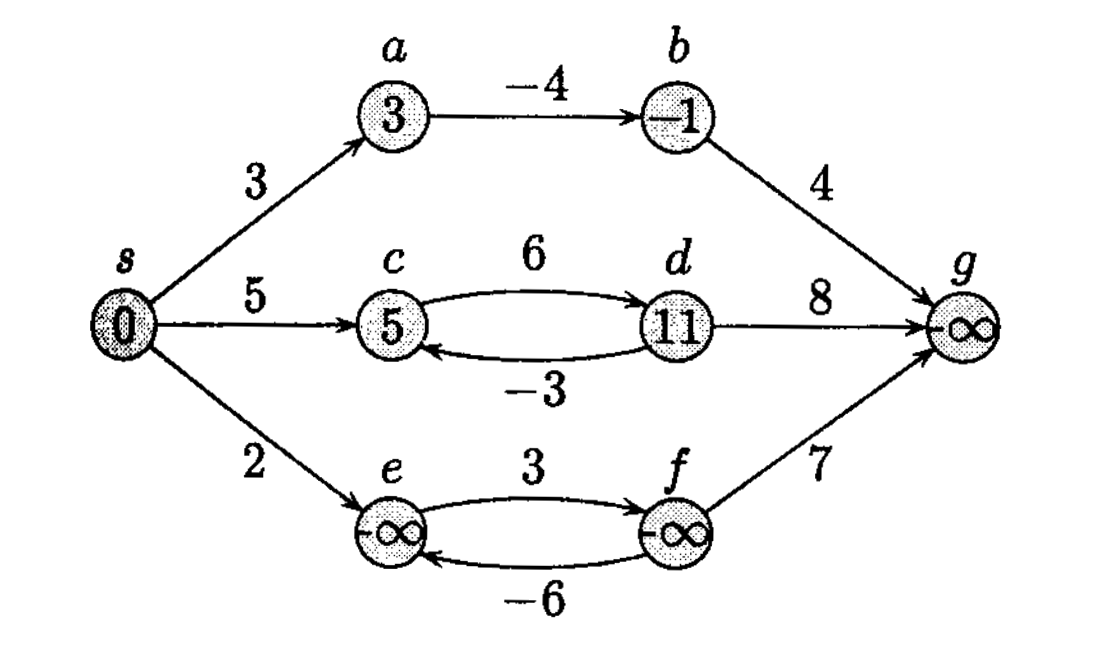
\includegraphics[width=1.0\linewidth]{images/closest1.png}}
\end{figure}
\end{frame}

\begin{frame}{Граф. Релаксация.}
\begin{figure}
\centerline{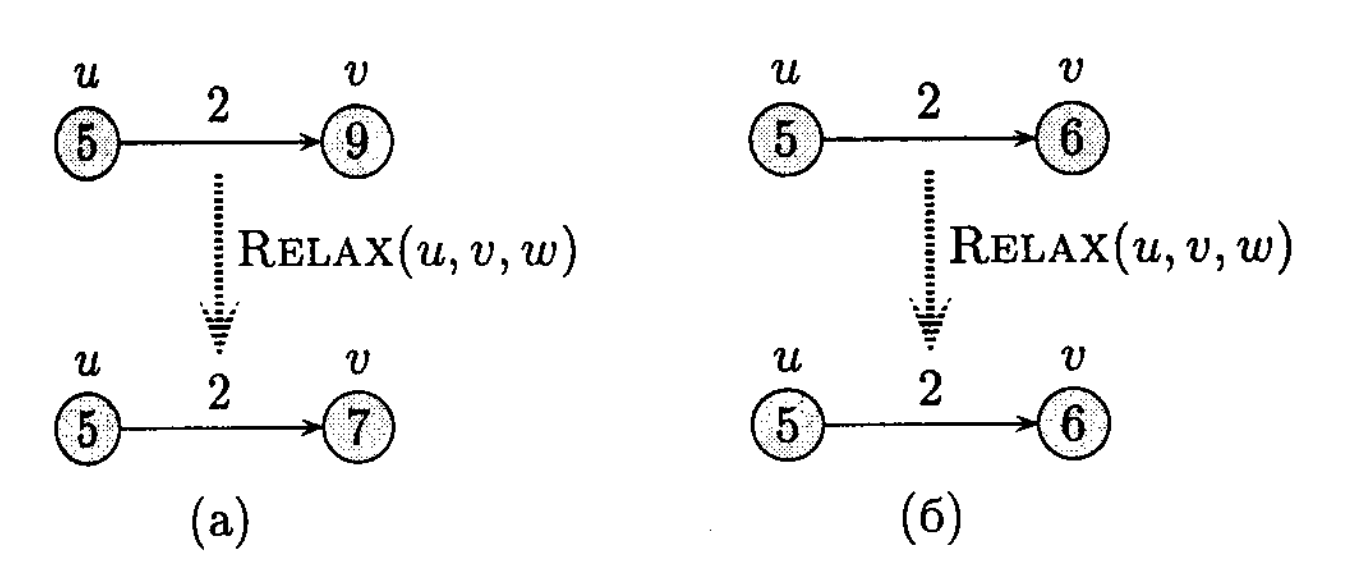
\includegraphics[width=1.0\linewidth]{images/relax.png}}
\end{figure}
\end{frame}

\begin{frame}{Граф. Алгоритм Дейкстры.}
\begin{figure}
\centerline{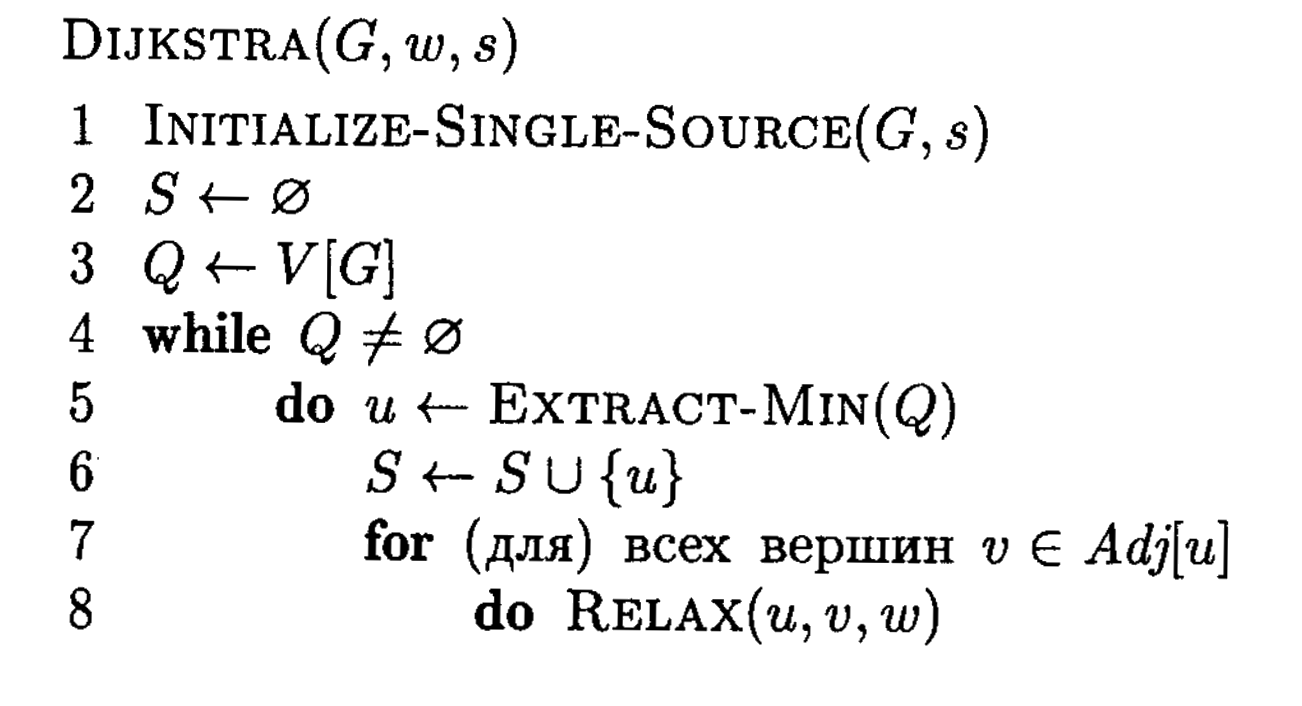
\includegraphics[width=1.0\linewidth]{images/deicstra_algo.png}}
\end{figure}
\end{frame}

\begin{frame}{Граф. Алгоритм Дейкстры.}
\begin{figure}
\centerline{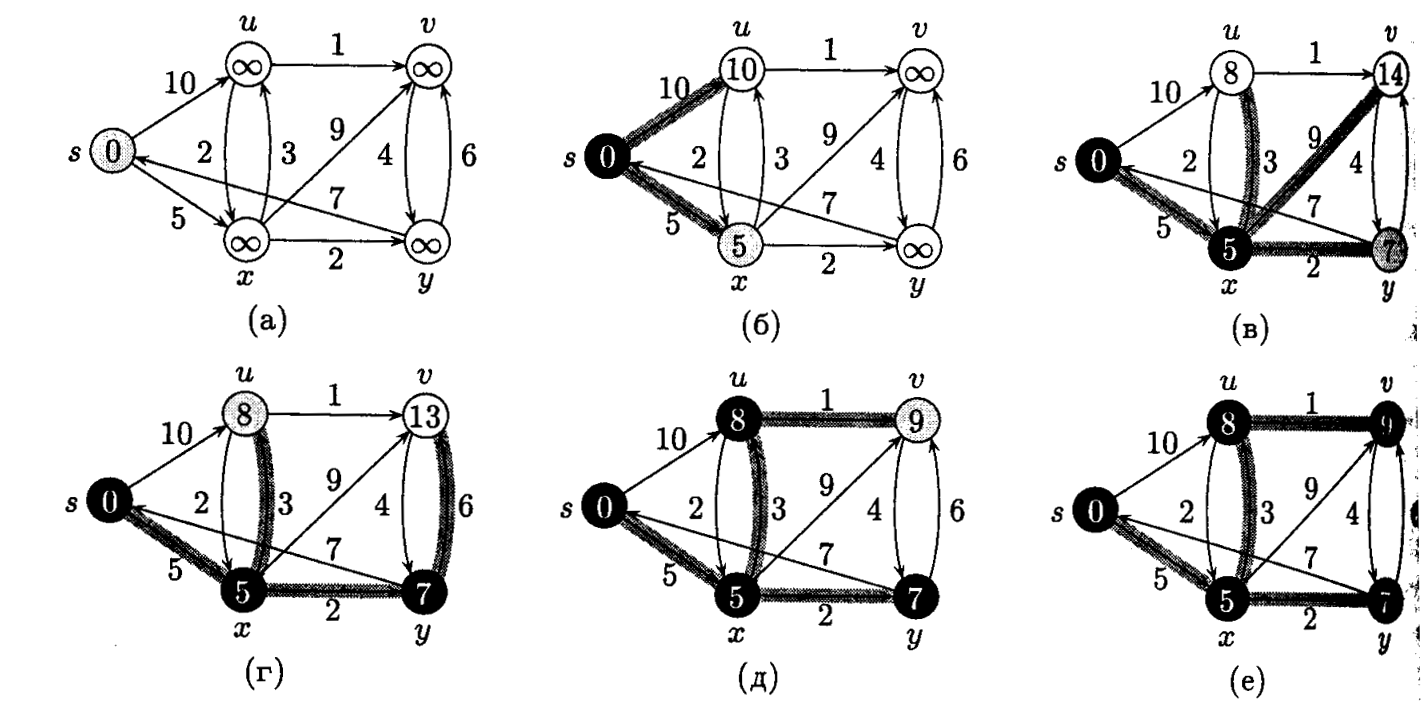
\includegraphics[width=1.0\linewidth]{images/deicstra_graphs.png}}
\end{figure}
\end{frame}



\begin{frame}{Граф. Сложности работы алгоритмов.}
\begin{itemize}
\item BFS -- $O(|V| + |E|)$
\item DFS -- $O(|V| + |E|)$
\item Алгоритм Дейкстры -- $O(|V|^2 + |E|)$
\item Алгоритм Беллмана-Форда -- $O(|V|*|E|)$ \\
(алгоритм нахождения кратчайших путей из одной вершины если есть отрицательные веса)
\item Алгоритм Флойда-Уоршолла -- $O(|V|^3)$ \\
(алгоритм нахождения кратчайших путей для всех пар вершин)
\end{itemize}
\end{frame}

%-=-=-=-=-=-=-=-=-=-=-=-=-=-=-=-=-=-=-=-=-=-=-=-=
%	Practical part:
%-=-=-=-=-=-=-=-=-=-=-=-=-=-=-=-=-=-=-=-=-=-=-=-=


\section{Практическая часть}






\end{document}